\documentclass[12pt, onecolumn]{article}

% 引入相关的包
\usepackage{amsmath, listings, fontspec, geometry, graphicx, ctex, color, subfigure, amsfonts, amssymb}
\usepackage{multirow}
\usepackage[table,xcdraw]{xcolor}
\usepackage[ruled]{algorithm2e}
\usepackage[hidelinks]{hyperref}

		\usepackage{graphicx}
		\usepackage[most]{tcolorbox}
\hypersetup{
	colorlinks=true,
	linkcolor=red,
	citecolor=red,
}
\usepackage{booktabs}
\usepackage{multirow}
\usepackage{picins}

% 设定页面的尺寸和比例
\geometry{left = 1.5cm, right = 1.5cm, top = 1.5cm, bottom = 1.5cm}

% 设定两栏之间的间距
\setlength\columnsep{1cm}

% 设定字体,为代码的插入作准备
\newfontfamily\ubuntu{Ubuntu Mono}
\newfontfamily\consolas{Consolas}

% 头部信息
\title{\normf{编程:观测值逐次更新的扩展卡尔曼滤波器}}
\author{\normf 姓名:陈烁龙\;\;\;学号:2023202140019\;\;\;学院:测绘学院}
\date{\normf{\today}}

% 代码块的风格设定
\lstset{
	language=C++,
	basicstyle=\small\ubuntu,
	keywordstyle=\textbf,
	stringstyle=\itshape,
	commentstyle=\itshape,
	numberstyle=\scriptsize\ubuntu,
	showstringspaces=false,
	numbers=left,
	numbersep=8pt,
	tabsize=2,
	frame=single,
	framerule=1pt,
	columns=fullflexible,
	breaklines,
	frame=shadowbox, 
	backgroundcolor=\color[rgb]{0.97,0.97,0.97}
}

% 字体族的定义
% \fangsong \songti \heiti \kaishu
\newcommand\normf{\fangsong}
\newcommand\boldf{\heiti}
\newcommand\keywords[1]{\bfseries{关键词:} \normf #1}

\newcommand\skewmat[1]{\left[ #1 \right]_\times}
\newcommand\liehat[1]{#1^{\land}}
\newcommand\lievee[1]{#1^\vee}
\newcommand\liehatvee[1]{\left[ #1 \right]^\vee_\times}

\newcommand\Exp[1]{\mathrm{Exp}\left( #1\right) }
\newcommand\Log[1]{\mathrm{Log}\left( #1\right) }

\newcommand\mlcomment[1]{\iffalse #1 \fi}
%\newcommand\mlcomment[1]{ #1 }

\newcommand\bsm[1]{\boldsymbol{\mathrm{#1}}}
\newcommand\rotation[2]{{\bsm{R}_{#1}^{#2}}}
\newcommand\quaternion[2]{{\bsm{q}_{#1}^{#2}}}
\newcommand\angvel[2]{{\bsm{\omega}_{#1}^{#2}}}
\newcommand\translation[2]{{\bsm{p}_{#1}^{#2}}}
\newcommand\translationhat[2]{{\hat{\bsm{p}}_{#1}^{#2}}}
\newcommand\linvel[2]{{\bsm{v}_{#1}^{#2}}}
\newcommand\linacce[2]{{\bsm{a}_{#1}^{#2}}}
\newcommand\gravity[1]{{\bsm{g}^{#1}}}
\newcommand\smallminus{{\text{-}}}
\newcommand\smallplus{{\text{+}}}
\newcommand\coordframe[1]{\underrightarrow{\mathcal{F}}_{#1}}

\newcounter{problemname}
\newenvironment{problem}{\stepcounter{problemname}\par\noindent\normf\textbf{\textcolor[rgb]{1,0,0}{题目\arabic{problemname}.} }}{\leavevmode\\\par}
\newenvironment{solution}{\par\noindent\normf\textbf{解答: }}{\leavevmode\\\par}
\newenvironment{note}{\par\noindent\normf\textbf{题目\arabic{problemname}的注记: }}{\leavevmode\\\par}


\begin{document}
	\begin{titlepage}
	    \centering
	    
\includegraphics[width=0.4\textwidth]{whu_red.png}\par\vspace{1cm}
	    \vspace{4cm}
	    {\huge\kaishu\bfseries Lie Group and Lie Algebra\par 李群李代数 \par}
	    \vspace{3cm}
	    {\Large\kaishu 
	    \begin{center}\begin{tabular}{l}
	    姓名:陈烁龙\\
	    学号:\bfseries 2023202140019\\
	    学院:测绘学院
	    \end{tabular}\end{center}
	     \par}
	    
	
	    \vfill
	
	% Bottom of the page
	    {\large\kaishu\bfseries \today\par}
	\end{titlepage}
		% 换页
 		\thispagestyle{empty}
		\clearpage
		
		% 插入目录、图、表并换页
		\pagenumbering{roman}
		\tableofcontents
		\newpage
		\listoffigures
%		\newpage
%		\listoftables
		% 罗马字母形式的页码
		
		\clearpage
		% 从该页开始计数
		\setcounter{page}{1}
		% 阿拉伯数字形式的页码
		\pagenumbering{arabic}
	
	\section{\normf{基础知识}}
	\normf\bfseries
	本文所有内容均来自于文献\cite{sola2018micro}。
	
	\begin{enumerate}
	\item 群运算:两个李群元素的李群运算结果仍然在群里。
	\begin{equation}
	\mathcal{X}\circ\mathcal{Y}\in\mathcal{G}
	\end{equation}
	
	\item 李代数(Lie algebra):流行$\mathcal{M}$上$\mathcal{X}$处的李代数为:
	\begin{equation}
	\mathfrak{m}=T_{\mathcal{X}}\mathcal{M}
	\end{equation}
	
	\item 指数运算和对数运算:
	\begin{equation}
	\mathcal{X}=\mathrm{Exp}(\bsm\tau)=\exp(\liehat{\bsm\tau})
	\qquad
	\bsm\tau=\mathrm{Log}(\mathcal{X})=\lievee{\log({\bsm\tau})}
	\end{equation}
	性质:
	\begin{equation}
	\exp\left( t\liehat{\bsm{\tau}}\right) =\exp\left(\liehat{\bsm{\tau}}\right) ^{t}
	\qquad
	\exp\left( \mathcal{X}\cdot\liehat{\bsm{\tau}}\cdot\mathcal{X}^{-1}\right) =
	\mathcal{X}\cdot\exp\left( \liehat{\bsm{\tau}}\right)\cdot\mathcal{X}^{-1}
	\end{equation}
	
	\item 加法和减法运算:
	\begin{enumerate}
	\item 右运算:
	\begin{equation}
	\mathcal{Y}=\mathcal{X}\oplus{^\mathcal{X}\bsm\tau}
	=\mathcal{X}\circ\Exp{{^\mathcal{X}\bsm\tau}}
	\qquad
	{^\mathcal{X}\bsm\tau}=\mathcal{Y}\ominus\mathcal{X}
	=\Log{\mathcal{X}^{-1}\circ\mathcal{Y}} 
	\end{equation}
	
	\item 左运算:
	\begin{equation}
	\mathcal{Y}={^\mathcal{E}\bsm\tau}\oplus\mathcal{X}
	=\Exp{{^\mathcal{E}\bsm\tau}}\circ\mathcal{X}
	\qquad
	{^\mathcal{E}\bsm\tau}=\mathcal{Y}\ominus\mathcal{X}
	=\Log{\mathcal{Y}\circ\mathcal{X}^{-1}} 
	\end{equation}
	\end{enumerate}
	
	\item 伴随和伴随矩阵:由于有:
	\begin{equation}
	\mathcal{Y}=\mathcal{X}\oplus{^\mathcal{X}\bsm\tau}={^\mathcal{E}\bsm\tau}\oplus\mathcal{X}
	\end{equation}
	所以${^\mathcal{X}\bsm\tau}$和${^\mathcal{E}\bsm\tau}$之间有转换关系:
	\begin{equation}
	\mathcal{X}\circ\Exp{{^\mathcal{X}\bsm\tau}}=\Exp{{^\mathcal{E}\bsm\tau}}\circ\mathcal{X}
	\qquad
	\Exp{{^\mathcal{E}\bsm\tau}}=\mathcal{X}\circ\Exp{{^\mathcal{X}\bsm\tau}}\circ\mathcal{X}^{-1}
	\end{equation}
	也即:
	\begin{equation}
	\liehat{{^\mathcal{E}\bsm\tau}}=\mathcal{X}\cdot\liehat{{^\mathcal{X}\bsm\tau}}\cdot\mathcal{X}^{-1}=\mathrm{Ad}_\mathcal{X}\left( \liehat{{\bsm\tau}}\right) 
	\end{equation}
	该变换是线性变换,所以可以写为矩阵乘法:
	\begin{equation}
	\liehat{{^\mathcal{E}\bsm\tau}}=\bsm{Ad}_\mathcal{X}\cdot\liehat{{\bsm\tau}}
	\qquad
	{^\mathcal{E}\bsm\tau}=\bsm{Ad}_\mathcal{X}\cdot{\bsm\tau}=
	\lievee{\left( \mathcal{X}\cdot\liehat{{^\mathcal{X}\bsm\tau}}\cdot\mathcal{X}^{-1}\right) }
	\end{equation}
	其中的$\bsm{Ad}_\mathcal{X}$即为$\mathcal{X}$处的伴随矩阵。有对应的性质:
	\begin{equation}
	\mathcal{X}\oplus\bsm{\tau}=(\bsm{Ad}_{\mathcal{X}}\cdot\bsm{\tau})\oplus\mathcal{X}
	\qquad
	\bsm{Ad}_{\mathcal{X}^{-1}}=\bsm{Ad}_{\mathcal{X}}^{-1}
	\qquad
	\bsm{Ad}_{\mathcal{X}\circ\mathcal{Y}}=\bsm{Ad}_{\mathcal{X}}\cdot\bsm{Ad}_{\mathcal{Y}}
	\end{equation}
	
	\item 李群上的雅克比:
	\begin{enumerate}
	\item 右雅克比:
	\begin{equation}
	\frac{{^\mathcal{X}Df(\mathcal{X})}}{D\mathcal{X}}
	=\lim\frac{f(\mathcal{X}\oplus\bsm{\tau})\ominus f(\mathcal{X})}{\bsm{\tau}}
	=\left. \frac{\partial \Log{f(\mathcal{X})^{-1}\circ f(\mathcal{X}\circ\Exp{\bsm\tau})}}{\partial \bsm{\tau}}\right|_{\bsm{\tau}=0}
	\end{equation}
	更新:
	\begin{equation}
	f(\mathcal{X}\oplus\bsm{\tau})=f(\mathcal{X})\oplus \frac{{^\mathcal{X}Df(\mathcal{X})}}{D\mathcal{X}}\cdot{^{\mathcal{X}}\bsm{\tau}}
	\end{equation}
	
	\item 左雅克比:
	\begin{equation}
	\frac{{^\mathcal{E}Df(\mathcal{X})}}{D\mathcal{X}}
	=\lim\frac{f(\bsm{\tau}\oplus\mathcal{X})\ominus f(\mathcal{X})}{\bsm{\tau}}
	=\left. \frac{\partial \Log{f(\Exp{\bsm\tau}\circ\mathcal{X})\circ f(\mathcal{X})^{-1}}}{\partial \bsm{\tau}}\right|_{\bsm{\tau}=0}
	\end{equation}
	更新:
	\begin{equation}
	f(\bsm{\tau}\oplus\mathcal{X})= \frac{{^\mathcal{E}Df(\mathcal{X})}}{D\mathcal{X}}\cdot{^{\mathcal{E}}\bsm{\tau}}
	\oplus f(\mathcal{X})
	\end{equation}
	
	\item 右雅克比转左雅克比:
	\begin{equation}
	\frac{{^\mathcal{E}Df(\mathcal{X})}}{D\mathcal{X}}=
	\bsm{Ad}_{f(\mathcal{X})}\cdot\frac{{^\mathcal{X}Df(\mathcal{X})}}{D\mathcal{X}}
	\cdot\bsm{Ad}_{\mathcal{X}}^{-1}
	\end{equation}
	\end{enumerate}
	
	\item 流形的雅克比:
	\begin{enumerate}
	\item 流形$\mathcal{M}$的右雅克比定义为李群$\mathcal{X}=\Exp{\bsm\tau}$的右雅克比:
	\begin{equation}
	\bsm{J}_r(\bsm\tau)=\frac{^{\bsm{\tau}}D\Exp{\bsm\tau}}{D\bsm\tau}\in\mathbb{R}^{m\times m}
	\end{equation}
	有常用性质:
	\begin{equation}
	\begin{aligned}
		\Exp{\bsm{\tau}+\delta\bsm{\tau}}&\approx\Exp{\bsm\tau}\circ\Exp{\bsm{J}_r(\bsm\tau)\delta\bsm{\tau}}
		\\
		\Exp{\bsm\tau}\circ\Exp{\delta\bsm\tau}&\approx\Exp{\bsm{\tau}+\bsm{J}_r^{-1}(\bsm\tau)\delta\bsm{\tau}}
		\\
		\Log{\Exp{\bsm\tau}\circ\Exp{\delta\bsm\tau}}&\approx\bsm{\tau}+\bsm{J}_r^{-1}(\bsm\tau)\delta\bsm{\tau}
	\end{aligned}
	\end{equation}	
	
	\item 流形$\mathcal{M}$的左雅克比定义为李群$\mathcal{X}=\Exp{\bsm\tau}$的左雅克比:
		\begin{equation}
		\bsm{J}_l(\bsm\tau)=\frac{^\mathcal{E}D\Exp{\bsm\tau}}{D\bsm\tau}\in\mathbb{R}^{m\times m}
		\end{equation}
	有常用性质:
	\begin{equation}
	\begin{aligned}
		\Exp{\bsm{\tau}+\delta\bsm{\tau}}&\approx\Exp{\bsm{J}_l(\bsm\tau)\delta\bsm{\tau}}\circ\Exp{\bsm\tau}
		\\
		\Exp{\delta\bsm\tau}\circ\Exp{\bsm\tau}&\approx\Exp{\bsm{\tau}+\bsm{J}_l^{-1}(\bsm\tau)\delta\bsm{\tau}}
		\\
		\Log{\Exp{\delta\bsm\tau}\circ\Exp{\bsm\tau}}&\approx\bsm{\tau}+\bsm{J}_l^{-1}(\bsm\tau)\delta\bsm{\tau}
	\end{aligned}
	\end{equation}	
	
	\item 对于两者,有:
	\begin{equation}
	\bsm{Ad}_{\Exp{\bsm{\tau}}}=\bsm{J}_l(\bsm\tau)\cdot\bsm{J}_r^{-1}(\bsm\tau)
	\end{equation}
	\begin{equation}
	\bsm{J}_r(-\bsm\tau)=\bsm{J}^{\Exp{-\bsm\tau}}_{-\bsm\tau}
	=\bsm{J}^{\Exp{\bsm\tau}^{-1}}_{\bsm\tau}\cdot\bsm{J}^{\bsm\tau}_{-\bsm\tau}
	=-\bsm{J}^{\Exp{\bsm\tau}^{-1}}_{\Exp{\bsm\tau}}\cdot\bsm{J}^{\Exp{\bsm\tau}}_{\bsm\tau}\cdot\bsm{I}
	=\bsm{Ad}_{\Exp{\bsm{\tau}}}\cdot\bsm{J}_r(\bsm\tau)=\bsm{J}_l(\bsm\tau)
	\end{equation}
	
	\item 另有:
	\begin{equation}
	\begin{aligned}
	^\mathcal{X}\bsm{J}^{\Log{\mathcal{X}}}_{\mathcal{\mathcal{X}}}&=
	\frac{\partial \left( \Log{\Exp{\bsm\tau}\circ\Exp{\delta\bsm\tau}}-\Log{\Exp{\bsm\tau}}\right)}{\partial \delta\bsm{\tau}}
	\\
	&=\frac{\partial \left( \bsm{\tau}+\bsm{J}_r^{-1}(\bsm\tau)\delta\bsm{\tau}-\bsm\tau\right)}{\partial \delta\bsm{\tau}}=\bsm{J}_r^{-1}(\bsm\tau)
	\end{aligned}
	\qquad
	^\mathcal{E}\bsm{J}^{\Log{\mathcal{X}}}_{\mathcal{\mathcal{X}}}
	=\bsm{J}_l^{-1}(\bsm\tau)
	\end{equation}
	\end{enumerate}
	
	\end{enumerate}
	
	\section{\normf 常用的雅克比}
	\subsection{\normf 右雅克比}
	\vspace{5mm}
	\begin{equation}
	\begin{aligned}
	\bsm{J}_{\mathcal{X}}^{\mathcal{X}}&=
	\left. \frac{\partial \Log{f(\mathcal{X})^{-1}\circ f(\mathcal{X}\circ\Exp{\bsm\tau})}}{\partial \bsm{\tau}}\right|_{\bsm{\tau}=0}
	\\&=\left. \frac{\partial \Log{\mathcal{X}^{-1}\circ \mathcal{X}\circ\Exp{\bsm\tau}}}{\partial \bsm{\tau}}\right|_{\bsm{\tau}=0}
	\\&=\left. \frac{\partial \Log{\Exp{\bsm\tau}}}{\partial \bsm{\tau}}\right|_{\bsm{\tau}=0}=\bsm{I}
	\end{aligned}
	\end{equation}
	\vspace{5mm}
	\begin{equation}
	\begin{aligned}
	\bsm{J}_{\mathcal{X}}^{\mathcal{X}^{-1}}&=
	\left. \frac{\partial \Log{f(\mathcal{X})^{-1}\circ f(\mathcal{X}\circ\Exp{\bsm\tau})}}{\partial \bsm{\tau}}\right|_{\bsm{\tau}=0}
	\\&=\left. \frac{
	\partial \Log{\mathcal{X}\circ\Exp{\bsm\tau}^{-1}\circ\mathcal{X}^{-1}}
	}{\partial \bsm{\tau}}\right|_{\bsm{\tau}=0}
	\\&=\left. \frac{
		\partial \Log{\Exp{-\mathcal{X}\cdot\liehat{\bsm\tau}\cdot\mathcal{X}^{-1}}}
		}{\partial \bsm{\tau}}\right|_{\bsm{\tau}=0}
	\\&=-\left. \frac{
		\partial \left( \mathcal{X}\cdot\liehat{\bsm\tau}\cdot\mathcal{X}^{-1}\right) 
		}{\partial \bsm{\tau}}\right|_{\bsm{\tau}=0}
	\\&=-\left. \frac{
		\partial \bsm{Ad}_{\mathcal{X}}\cdot\bsm{\tau} 
		}{\partial \bsm{\tau}}\right|_{\bsm{\tau}=0}=-\bsm{Ad}_{\mathcal{X}}
	\end{aligned}
	\end{equation}
	\vspace{5mm}
	\begin{equation}
	\begin{aligned}
	\bsm{J}_{\mathcal{X}}^{\mathcal{X}\circ\mathcal{Y}}&=
	\left. \frac{\partial \Log{f(\mathcal{X})^{-1}\circ f(\mathcal{X}\circ\Exp{\bsm\tau})}}{\partial \bsm{\tau}}\right|_{\bsm{\tau}=0}
	\\&=\left. \frac{\partial \Log{\mathcal{Y}^{-1}\circ\mathcal{X}^{-1}\circ \mathcal{X}\circ\Exp{\bsm\tau}\circ\mathcal{Y}}}{\partial \bsm{\tau}}\right|_{\bsm{\tau}=0}
	\\&=\left. \frac{\partial \Log{\mathcal{Y}^{-1}\circ\Exp{\bsm\tau}\circ\mathcal{Y}}}{\partial \bsm{\tau}}\right|_{\bsm{\tau}=0}
	\\&=\left. \frac{\partial \left( \mathcal{Y}^{-1}\cdot\liehat{\bsm{\tau}}\cdot\mathcal{Y}\right) }{\partial \bsm{\tau}}\right|_{\bsm{\tau}=0}
	\\&=\left. \frac{\partial \bsm{Ad}_{\mathcal{Y}^{-1}}\cdot\bsm{\tau} }{\partial \bsm{\tau}}\right|_{\bsm{\tau}=0}=\bsm{Ad}_{\mathcal{Y}^{-1}}=\bsm{Ad}_{\mathcal{Y}}^{-1}
	\end{aligned}
	\end{equation}
	\vspace{5mm}
	\begin{equation}
	\begin{aligned}
	\bsm{J}_{\mathcal{X}}^{\mathcal{Y}\circ\mathcal{X}}&=
	\left. \frac{\partial \Log{f(\mathcal{X})^{-1}\circ f(\mathcal{X}\circ\Exp{\bsm\tau})}}{\partial \bsm{\tau}}\right|_{\bsm{\tau}=0}
	\\&=	\left. \frac{\partial \Log{\mathcal{X}^{-1}\cdot\mathcal{Y}^{-1}\circ \mathcal{Y}\circ\mathcal{X}\circ\Exp{\bsm\tau}}}{\partial \bsm{\tau}}\right|_{\bsm{\tau}=0}
	\\&=	\left. \frac{\partial \Log{\Exp{\bsm\tau}}}{\partial \bsm{\tau}}\right|_{\bsm{\tau}=0}=\bsm{I}
	\end{aligned}
	\end{equation}
	\vspace{5mm}
	\begin{equation}
	\bsm{J}_{\mathcal{X}}^{\mathcal{X}^{-1}\circ\mathcal{Y}}=
	\bsm{J}_{\mathcal{X}^{-1}}^{\mathcal{X}^{-1}\circ\mathcal{Y}}\cdot
	\bsm{J}_{\mathcal{X}}^{\mathcal{X}^{-1}}
	=\bsm{Ad}_{\mathcal{Y}}^{-1}\cdot\left( -\bsm{Ad}_{\mathcal{X}}\right) 
	=-\bsm{Ad}_{\mathcal{Y}}^{-1}\cdot\bsm{Ad}_{\mathcal{X}}
	\end{equation}
	\vspace{5mm}
	\begin{equation}
	\bsm{J}_{\mathcal{X}}^{\mathcal{Y}\circ\mathcal{X}^{-1}}=
	\bsm{J}_{\mathcal{X}^{-1}}^{\mathcal{Y}\circ\mathcal{X}^{-1}}\cdot
	\bsm{J}_{\mathcal{X}}^{\mathcal{X}^{-1}}
	=\bsm{I}\cdot\left( -\bsm{Ad}_{\mathcal{X}}\right) =-\bsm{Ad}_{\mathcal{X}}
	\end{equation}
	\vspace{5mm}
	\begin{equation}
	\bsm{J}_{\mathcal{X}}^{\mathcal{Y}\circ\mathcal{X}\circ\mathcal{Z}}=
	\bsm{J}_{\mathcal{X}\circ\mathcal{Z}}^{\mathcal{Y}\circ\mathcal{X}\circ\mathcal{Z}}\cdot\bsm{J}_{\mathcal{X}}^{\mathcal{X}\circ\mathcal{Z}}
	=\bsm{I}\cdot\bsm{Ad}_{\mathcal{Z}}^{-1}=\bsm{Ad}_{\mathcal{Z}}^{-1}
	\end{equation}
	\vspace{5mm}
	\begin{equation}
	\bsm{J}_{\mathcal{X}}^{\mathcal{Y}\circ\mathcal{X}^{-1}\circ\mathcal{Z}}=
	\bsm{J}_{\mathcal{X}^{-1}\circ\mathcal{Z}}^{\mathcal{Y}\circ\mathcal{X}^{-1}\circ\mathcal{Z}}\cdot\bsm{J}_{\mathcal{X}}^{\mathcal{X}^{-1}\circ\mathcal{Z}}
	=\bsm{I}\cdot\left( -\bsm{Ad}_{\mathcal{Z}}^{-1}\cdot\bsm{Ad}_{\mathcal{X}}\right)
	= -\bsm{Ad}_{\mathcal{Z}}^{-1}\cdot\bsm{Ad}_{\mathcal{X}}
	\end{equation}
	
	\subsection{\normf 左雅克比}
	基于公式:
	\begin{equation}
	\frac{{^\mathcal{E}Df(\mathcal{X})}}{D\mathcal{X}}=
	\bsm{Ad}_{f(\mathcal{X})}\cdot\frac{{^\mathcal{X}Df(\mathcal{X})}}{D\mathcal{X}}
	\cdot\bsm{Ad}_{\mathcal{X}}^{-1}
	\end{equation}
	可以从右雅克比得到对应的左雅克比:
	\begin{equation}
	^\mathcal{E}\bsm{J}_{\mathcal{X}}^{\mathcal{X}}
	=\bsm{Ad}_{\mathcal{X}}\cdot\bsm{J}_{\mathcal{X}}^{\mathcal{X}}\cdot\bsm{Ad}_{\mathcal{X}}^{-1}=\bsm{Ad}_{\mathcal{X}}\cdot\bsm{Ad}_{\mathcal{X}}^{-1}=\bsm{I}
	\end{equation}
	\begin{equation}
	^\mathcal{E}\bsm{J}_{\mathcal{X}}^{\mathcal{X}^{-1}}
	=\bsm{Ad}_{\mathcal{X}}^{-1}\cdot\bsm{J}_{\mathcal{X}}^{\mathcal{X}^{-1}}\cdot\bsm{Ad}_{\mathcal{X}}^{-1}
	=\bsm{Ad}_{\mathcal{X}}^{-1}\cdot\left( -\bsm{Ad}_{\mathcal{X}}\right) \cdot\bsm{Ad}_{\mathcal{X}}^{-1}=-\bsm{Ad}_{\mathcal{X}}^{-1}
	\end{equation}
	\begin{equation}
	^\mathcal{E}\bsm{J}_{\mathcal{X}}^{\mathcal{X}\circ\mathcal{Y}}
	=\bsm{Ad}_{\mathcal{X}}\cdot\bsm{Ad}_{\mathcal{Y}}\cdot
	\bsm{J}_{\mathcal{X}}^{\mathcal{X}\circ\mathcal{Y}}\cdot\bsm{Ad}_{\mathcal{X}}^{-1}
	=\bsm{Ad}_{\mathcal{X}}\cdot\bsm{Ad}_{\mathcal{Y}}\cdot
	\bsm{Ad}_{\mathcal{Y}}^{-1}\cdot\bsm{Ad}_{\mathcal{X}}^{-1}=\bsm{I}
	\end{equation}
	\begin{equation}
	^\mathcal{E}\bsm{J}_{\mathcal{X}}^{\mathcal{Y}\circ\mathcal{X}}
	=\bsm{Ad}_{\mathcal{Y}}\cdot\bsm{Ad}_{\mathcal{X}}\cdot
	\bsm{J}_{\mathcal{X}}^{\mathcal{Y}\circ\mathcal{X}}\cdot\bsm{Ad}_{\mathcal{X}}^{-1}
	=\bsm{Ad}_{\mathcal{Y}}\cdot\bsm{Ad}_{\mathcal{X}}\cdot
	\bsm{Ad}_{\mathcal{X}}^{-1}=\bsm{Ad}_{\mathcal{Y}}
	\end{equation}
	\begin{equation}
	^\mathcal{E}\bsm{J}_{\mathcal{X}}^{\mathcal{X}^{-1}\circ\mathcal{Y}}
	=\bsm{Ad}_{\mathcal{X}}^{-1}\cdot\bsm{Ad}_{\mathcal{Y}}\cdot
	\bsm{J}_{\mathcal{X}}^{\mathcal{X}^{-1}\circ\mathcal{Y}}\cdot\bsm{Ad}_{\mathcal{X}}^{-1}
	=\bsm{Ad}_{\mathcal{X}}^{-1}\cdot\bsm{Ad}_{\mathcal{Y}}\cdot
	\left( -\bsm{Ad}_{\mathcal{Y}}^{-1}\cdot\bsm{Ad}_{\mathcal{X}}\right) \cdot\bsm{Ad}_{\mathcal{X}}^{-1}=-\bsm{Ad}_{\mathcal{X}}^{-1}
	\end{equation}
	\begin{equation}
	^\mathcal{E}\bsm{J}_{\mathcal{X}}^{\mathcal{Y}\circ\mathcal{X}^{-1}}
	=\bsm{Ad}_{\mathcal{Y}}\cdot\bsm{Ad}_{\mathcal{X}}^{-1}\cdot
	\bsm{J}_{\mathcal{X}}^{\mathcal{Y}\circ\mathcal{X}^{-1}}\cdot
	\bsm{Ad}_{\mathcal{X}}^{-1}
	=\bsm{Ad}_{\mathcal{Y}}\cdot\bsm{Ad}_{\mathcal{X}}^{-1}\cdot
		\left( -\bsm{Ad}_{\mathcal{X}}\right) \cdot
		\bsm{Ad}_{\mathcal{X}}^{-1}=-\bsm{Ad}_{\mathcal{Y}}\cdot\bsm{Ad}_{\mathcal{X}}^{-1}
	\end{equation}
	\begin{equation}
	^\mathcal{E}\bsm{J}_{\mathcal{X}}^{\mathcal{Y}\circ\mathcal{X}\circ\mathcal{Z}}
	=\bsm{Ad}_{\mathcal{Y}}\cdot\bsm{Ad}_{\mathcal{X}}\cdot\bsm{Ad}_{\mathcal{Z}}\cdot
	\bsm{J}_{\mathcal{X}}^{\mathcal{Y}\circ\mathcal{X}\circ\mathcal{Z}}\cdot
	\bsm{Ad}_{\mathcal{X}}^{-1}
	=\bsm{Ad}_{\mathcal{Y}}\cdot\bsm{Ad}_{\mathcal{X}}\cdot\bsm{Ad}_{\mathcal{Z}}\cdot
		\bsm{Ad}_{\mathcal{Z}}^{-1}\cdot
		\bsm{Ad}_{\mathcal{X}}^{-1}
		=\bsm{Ad}_{\mathcal{Y}}
	\end{equation}
	\begin{equation}
	^\mathcal{E}\bsm{J}_{\mathcal{X}}^{\mathcal{Y}\circ\mathcal{X}^{-1}\circ\mathcal{Z}}
	=\bsm{Ad}_{\mathcal{Y}}\cdot\bsm{Ad}_{\mathcal{X}}^{-1}\cdot\bsm{Ad}_{\mathcal{Z}}\cdot\bsm{J}_{\mathcal{X}}^{\mathcal{Y}\circ\mathcal{X}^{-1}\circ\mathcal{Z}}\cdot
	\bsm{Ad}_{\mathcal{X}}^{-1}
	=\bsm{Ad}_{\mathcal{Y}}\cdot\bsm{Ad}_{\mathcal{X}}^{-1}\cdot\bsm{Ad}_{\mathcal{Z}}\cdot\left( 
	-\bsm{Ad}_{\mathcal{Z}}^{-1}\cdot\bsm{Ad}_{\mathcal{X}}\right) \cdot
		\bsm{Ad}_{\mathcal{X}}^{-1}
		=-\bsm{Ad}_{\mathcal{Y}}\cdot\bsm{Ad}_{\mathcal{X}}^{-1}
	\end{equation}
	
	\subsection{\normf 整理}
	\begin{enumerate}
	\item 右雅克比
	\begin{equation}
	\begin{gathered}
	\bsm{J}_{\mathcal{X}}^{\mathcal{X}}=\bsm{I}
	\qquad
	\bsm{J}_{\mathcal{X}}^{\mathcal{X}^{-1}}=-\bsm{Ad}_{\mathcal{X}}
	\qquad
	\bsm{J}_{\mathcal{X}}^{\mathcal{X}\circ\mathcal{Y}}=\bsm{Ad}_{\mathcal{Y}}^{-1}
	\qquad
	\bsm{J}_{\mathcal{X}}^{\mathcal{Y}\circ\mathcal{X}}=\bsm{I}
	\qquad
	\bsm{J}_{\mathcal{X}}^{\mathcal{X}^{-1}\circ\mathcal{Y}}=-\bsm{Ad}_{\mathcal{Y}}^{-1}\cdot\bsm{Ad}_{\mathcal{X}}
	\\
	\bsm{J}_{\mathcal{X}}^{\mathcal{Y}\circ\mathcal{X}^{-1}}=-\bsm{Ad}_{\mathcal{X}}
	\qquad
	\bsm{J}_{\mathcal{X}}^{\mathcal{Y}\circ\mathcal{X}\circ\mathcal{Z}}=\bsm{Ad}_{\mathcal{Z}}^{-1}
	\qquad
	\bsm{J}_{\mathcal{X}}^{\mathcal{Y}\circ\mathcal{X}^{-1}\circ\mathcal{Z}}=
	-\bsm{Ad}_{\mathcal{Z}}^{-1}\cdot\bsm{Ad}_{\mathcal{X}}
	\end{gathered}
	\end{equation}

	\item 左雅克比
	\begin{equation}
	\begin{gathered}
	^\mathcal{E}\bsm{J}_{\mathcal{X}}^{\mathcal{X}}=\bsm{I}
	\qquad
	^\mathcal{E}\bsm{J}_{\mathcal{X}}^{\mathcal{X}^{-1}}=-\bsm{Ad}_{\mathcal{X}}^{-1}
	\qquad
	^\mathcal{E}\bsm{J}_{\mathcal{X}}^{\mathcal{X}\circ\mathcal{Y}}=\bsm{I}
	\qquad
	^\mathcal{E}\bsm{J}_{\mathcal{X}}^{\mathcal{Y}\circ\mathcal{X}}=\bsm{Ad}_{\mathcal{Y}}
	\qquad
	^\mathcal{E}\bsm{J}_{\mathcal{X}}^{\mathcal{X}^{-1}\circ\mathcal{Y}}=-\bsm{Ad}_{\mathcal{X}}^{-1}
	\\
	^\mathcal{E}\bsm{J}_{\mathcal{X}}^{\mathcal{Y}\circ\mathcal{X}^{-1}}=-\bsm{Ad}_{\mathcal{Y}}\cdot\bsm{Ad}_{\mathcal{X}}^{-1}
	\qquad
	^\mathcal{E}\bsm{J}_{\mathcal{X}}^{\mathcal{Y}\circ\mathcal{X}\circ\mathcal{Z}}=\bsm{Ad}_{\mathcal{Y}}
	\qquad
	^\mathcal{E}\bsm{J}_{\mathcal{X}}^{\mathcal{Y}\circ\mathcal{X}^{-1}\circ\mathcal{Z}}=-\bsm{Ad}_{\mathcal{Y}}\cdot\bsm{Ad}_{\mathcal{X}}^{-1}
	\end{gathered}
	\end{equation}
	\end{enumerate}
	
	\section{\normf 二维旋转群SO(2)}
	有:
	\begin{equation}
	\bsm{R}=\begin{bmatrix}
	\cos\theta&-\sin\theta\\
	\sin\theta&\cos\theta
	\end{bmatrix}
	\qquad
	\liehat{\bsm{\tau}}=\liehat{\theta}=\skewmat{{\theta}}=\begin{bmatrix}
	0&-\theta\\
	\theta&0
	\end{bmatrix}
	\qquad
	\bsm{Ad}_{\bsm{R}}\cdot\theta=\lievee{\left(\bsm{R}\cdot\liehat{\theta}\cdot\bsm{R}^\top \right) }=\theta
	\qquad
	\bsm{Ad}_{\bsm{R}}=1
	\end{equation}
	推导:
	\begin{equation}
	\bsm{R}\cdot\liehat{\theta}\cdot\bsm{R}^\top =
	\begin{bmatrix}
		\cos\theta&-\sin\theta\\
		\sin\theta&\cos\theta
		\end{bmatrix}\begin{bmatrix}
			0&-\theta\\
			\theta&0
			\end{bmatrix}\begin{bmatrix}
					\cos\theta&\sin\theta\\
					-\sin\theta&\cos\theta
					\end{bmatrix}=\begin{bmatrix}
						0&-\theta\\
						\theta&0
						\end{bmatrix}
	\end{equation}
	于是得到:
	\begin{enumerate}
	\item 右雅克比
	\begin{equation}
	\begin{gathered}
	\bsm{J}_{\bsm{R}}^{\bsm{R}}=1
	\qquad
	\bsm{J}_{\bsm{R}}^{\bsm{R}^{-1}}=-1
	\qquad
	\bsm{J}_{\bsm{R}}^{\bsm{R}\cdot\bsm{Q}}=1
	\qquad
	\bsm{J}_{\bsm{R}}^{\bsm{Q}\cdot\bsm{R}}=1
	\qquad
	\bsm{J}_{\bsm{R}}^{\bsm{R}^{-1}\cdot\bsm{Q}}=-1
	\\
	\bsm{J}_{\bsm{R}}^{\bsm{Q}\cdot\bsm{R}^{-1}}=-1
	\qquad
	\bsm{J}_{\bsm{R}}^{\bsm{Q}\cdot\bsm{R}\cdot\bsm{P}}=1
	\qquad
	\bsm{J}_{\bsm{R}}^{\bsm{Q}\cdot\bsm{R}^{-1}\cdot\bsm{P}}=-1
	\end{gathered}
	\end{equation}

	\item 左雅克比
	\begin{equation}
	\begin{gathered}
	^\mathcal{E}\bsm{J}_{\bsm{R}}^{\bsm{R}}=1
	\qquad
	^\mathcal{E}\bsm{J}_{\bsm{R}}^{\bsm{R}^{-1}}=-1
	\qquad
	^\mathcal{E}\bsm{J}_{\bsm{R}}^{\bsm{R}\cdot\bsm{Q}}=1
	\qquad
	^\mathcal{E}\bsm{J}_{\bsm{R}}^{\bsm{Q}\cdot\bsm{R}}=1
	\qquad
	^\mathcal{E}\bsm{J}_{\bsm{R}}^{\bsm{R}^{-1}\cdot\bsm{Q}}=-1
	\\
	^\mathcal{E}\bsm{J}_{\bsm{R}}^{\bsm{Q}\cdot\bsm{R}^{-1}}=-1
	\qquad
	^\mathcal{E}\bsm{J}_{\bsm{R}}^{\bsm{Q}\cdot\bsm{R}\cdot\bsm{P}}=1
	\qquad
	^\mathcal{E}\bsm{J}_{\bsm{R}}^{\bsm{Q}\cdot\bsm{R}^{-1}\cdot\bsm{P}}=-1
	\end{gathered}
	\end{equation}
	\end{enumerate}
	特别的,对于向量$\bsm{v}$的操作,有右雅克比矩阵:
	\begin{equation}
	\begin{aligned}
	\bsm{J}_{\bsm{R}}^{\bsm{R}\cdot\bsm{v}}&=
	\lim\frac{\left( \bsm{R}\oplus\bsm{\tau}\right) \cdot\bsm{v}- \bsm{R}\cdot\bsm{v}}{\bsm{\tau}}=
	\lim\frac{\bsm{R}\cdot\Exp{\bsm{\tau}} \cdot\bsm{v}- \bsm{R}\cdot\bsm{v}}{\bsm{\tau}}
	\\
	&=\lim\frac{\bsm{R}\cdot\left( \bsm{I}+\liehat{\bsm{\tau}}\right)  \cdot\bsm{v}- \bsm{R}\cdot\bsm{v}}{\bsm{\tau}}
	=\lim\frac{\bsm{R}\cdot\liehat{\bsm{\tau}}  \cdot\bsm{v}}{\bsm{\tau}}
	=\bsm{R}\cdot\liehat{{1}}\cdot\bsm{v}
	\end{aligned}
	\end{equation}
	和左雅克比矩阵:
	\begin{equation}
	\begin{aligned}
	^\mathcal{E}\bsm{J}_{\bsm{R}}^{\bsm{R}\cdot\bsm{v}}&=
	\lim\frac{\left( \bsm{\tau}\oplus\bsm{R}\right) \cdot\bsm{v}- \bsm{R}\cdot\bsm{v}}{\bsm{\tau}}=
	\lim\frac{\Exp{\bsm{\tau}} \cdot\bsm{R}\cdot\bsm{v}- \bsm{R}\cdot\bsm{v}}{\bsm{\tau}}
	\\
	&=\lim\frac{\left( \bsm{I}+\liehat{\bsm{\tau}}\right)  \cdot\bsm{R}\cdot\bsm{v}- \bsm{R}\cdot\bsm{v}}{\bsm{\tau}}
	=\lim\frac{\liehat{\bsm{\tau}}  \cdot\bsm{R}\cdot\bsm{v}}{\bsm{\tau}}
	=\liehat{{1}}\cdot\bsm{R}\cdot\bsm{v}
	=\bsm{R}\cdot\liehat{{1}}\cdot\bsm{v}
	\end{aligned}
	\end{equation}
	也可以通过如下推导得到:
	\begin{equation}
	^\mathcal{E}\bsm{J}_{\bsm{R}}^{\bsm{R}\cdot\bsm{v}}=
	\bsm{Ad}_{f(\mathcal{X})}\cdot\frac{{^\mathcal{X}Df(\mathcal{X})}}{D\mathcal{X}}
		\cdot\bsm{Ad}_{\mathcal{X}}^{-1}
		=\bsm{I}_2\cdot\left(\bsm{R}\cdot\liehat{{1}}\cdot\bsm{v} \right) \cdot 1
		=\bsm{R}\cdot\liehat{{1}}\cdot\bsm{v}=\liehat{{1}}\cdot\bsm{R}\cdot\bsm{v}
	\end{equation}
	
	
	\section{\normf 二维刚体运动群SE(2)}
	有:
	\begin{equation}
	\bsm{M}=\begin{bmatrix}
	\bsm{R}&\bsm{t}\\
	\bsm{0}&1
	\end{bmatrix}
	\qquad
	\liehat{\bsm{\tau}}=\skewmat{\bsm{\tau}}=\begin{bmatrix}
	\liehat{\theta}&\bsm{\rho}\\
	\bsm{0}&0
	\end{bmatrix}\in\mathfrak{se}(2)
	\qquad
	\bsm{\tau}=\begin{bmatrix}
	\bsm{\rho}\\\theta
	\end{bmatrix}\in\mathbb{R}^3
	\qquad
	\bsm{Ad}_{\bsm{M}}\cdot\bsm{\tau}=\lievee{\left(\bsm{M}\cdot\liehat{\bsm{\tau}}\cdot\bsm{M}^{-1} \right) }
	\end{equation}
	有:
	\begin{equation}	
	\bsm{M}\cdot\liehat{\bsm{\tau}}\cdot\bsm{M}^{-1}=
	\begin{bmatrix}
		\bsm{R}&\bsm{t}\\
		\bsm{0}&1
		\end{bmatrix}\begin{bmatrix}
			\liehat{\theta}&\bsm{\rho}\\
			\bsm{0}&0
			\end{bmatrix}	\begin{bmatrix}
					\bsm{R}^\top&-\bsm{R}^\top\cdot\bsm{t}\\
					\bsm{0}&1
					\end{bmatrix}=\begin{bmatrix}
					\bsm{R}\cdot\liehat{\theta}\cdot\bsm{R}^\top&\bsm{R}\cdot\bsm{\rho}-\bsm{R}\cdot\liehat{\theta}\cdot\bsm{R}^\top\cdot\bsm{t}\\
					\bsm{0}&1
					\end{bmatrix}
	\end{equation}
	得到:
	\begin{equation}
	\lievee{\left(\bsm{M}\cdot\liehat{\bsm{\tau}}\cdot\bsm{M}^{-1} \right) }=
	\begin{bmatrix}
	\bsm{R}\cdot\bsm{\rho}-\liehat{\left( \bsm{Ad}_{\bsm{R}}\cdot\theta\right) }\cdot\bsm{t}\\
	\bsm{Ad}_{\bsm{R}}\cdot\theta
	\end{bmatrix}=	\begin{bmatrix}
		\bsm{R}\cdot\bsm{\rho}-\liehat{\theta}\cdot\bsm{t}\\
		\theta
		\end{bmatrix}=\begin{bmatrix}
		\bsm{R}&-\liehat{1}\cdot\bsm{t}\\
		\bsm{0}&1
		\end{bmatrix}\begin{bmatrix}
			\bsm{\rho}\\\theta
			\end{bmatrix}
	\end{equation}
	所以:
	\begin{equation}
	\bsm{Ad}_{\bsm{M}}=\begin{bmatrix}
			\bsm{R}&-\liehat{1}\cdot\bsm{t}\\
			\bsm{0}&1
			\end{bmatrix}
	\qquad
	\bsm{Ad}_{\bsm{M}}^{-1}=\begin{bmatrix}
			 			\bsm{R}^\top&\bsm{R}^\top\cdot\liehat{1}\cdot\bsm{t}\\
			 			\bsm{0}&1
			 			\end{bmatrix}
	\end{equation}
	于是得到:
	\begin{enumerate}
	\item 右雅克比
	\begin{equation}
	\begin{gathered}
	\bsm{J}_{\bsm{M}}^{\bsm{M}}=\bsm{I}_4
	\qquad
	\bsm{J}_{\bsm{M}}^{\bsm{M}^{-1}}=-\bsm{Ad}_{\bsm{M}}
	\qquad
	\bsm{J}_{\bsm{M}}^{\bsm{M}\cdot\bsm{N}}=\bsm{Ad}_{\bsm{N}}^{-1}
	\qquad
	\bsm{J}_{\bsm{M}}^{\bsm{N}\cdot\bsm{M}}=\bsm{I}_4
	\qquad
	\bsm{J}_{\bsm{M}}^{\bsm{M}^{-1}\cdot\bsm{N}}=-\bsm{Ad}_{\bsm{N}}^{-1}\cdot\bsm{Ad}_{\bsm{M}}
	\\
	\bsm{J}_{\bsm{M}}^{\bsm{N}\cdot\bsm{M}^{-1}}=-\bsm{Ad}_{\bsm{M}}
	\qquad
	\bsm{J}_{\bsm{M}}^{\bsm{N}\cdot\bsm{M}\cdot\bsm{L}}=\bsm{Ad}_{\bsm{L}}^{-1}
	\qquad
	\bsm{J}_{\bsm{M}}^{\bsm{N}\cdot\bsm{M}^{-1}\cdot\bsm{L}}=
	-\bsm{Ad}_{\bsm{L}}^{-1}\cdot\bsm{Ad}_{\bsm{M}}
	\end{gathered}
	\end{equation}

	\item 左雅克比
	\begin{equation}
	\begin{gathered}
	^\mathcal{E}\bsm{J}_{\bsm{M}}^{\bsm{M}}=\bsm{I}_4
	\qquad
	^\mathcal{E}\bsm{J}_{\bsm{M}}^{\bsm{M}^{-1}}=-\bsm{Ad}_{\bsm{M}}^{-1}
	\qquad
	^\mathcal{E}\bsm{J}_{\bsm{M}}^{\bsm{M}\cdot\bsm{N}}=\bsm{I}_4
	\qquad
	^\mathcal{E}\bsm{J}_{\bsm{M}}^{\bsm{N}\cdot\bsm{M}}=\bsm{Ad}_{\bsm{N}}
	\qquad
	^\mathcal{E}\bsm{J}_{\bsm{M}}^{\bsm{M}^{-1}\cdot\bsm{N}}=-\bsm{Ad}_{\bsm{M}}^{-1}
	\\
	^\mathcal{E}\bsm{J}_{\bsm{M}}^{\bsm{N}\cdot\bsm{M}^{-1}}=-\bsm{Ad}_{\bsm{N}}\cdot\bsm{Ad}_{\bsm{M}}^{-1}
	\qquad
	^\mathcal{E}\bsm{J}_{\bsm{M}}^{\bsm{N}\cdot\bsm{M}\cdot\bsm{L}}=\bsm{Ad}_{\bsm{N}}
	\qquad
	^\mathcal{E}\bsm{J}_{\bsm{M}}^{\bsm{N}\cdot\bsm{M}^{-1}\cdot\bsm{L}}=-\bsm{Ad}_{\bsm{N}}\cdot\bsm{Ad}_{\bsm{M}}^{-1}
	\end{gathered}
	\end{equation}
	\end{enumerate}
	特别的,对于点$\bsm{p}$的操作,有右雅克比矩阵:
	\begin{equation}
	\begin{aligned}
	\bsm{J}_{\bsm{M}}^{\bsm{M}\cdot\bsm{p}}&=
	\lim\frac{\left( \bsm{M}\oplus\bsm{\tau}\right) \cdot\bsm{p}- \bsm{M}\cdot\bsm{p}}{\bsm{\tau}}=
	\lim\frac{\bsm{M}\cdot\Exp{\bsm{\tau}} \cdot\bsm{p}- \bsm{M}\cdot\bsm{p}}{\bsm{\tau}}
	=\lim\frac{\bsm{M}\cdot\left( \bsm{I}+\liehat{\bsm{\tau}}\right)  \cdot\bsm{p}- \bsm{M}\cdot\bsm{p}}{\bsm{\tau}}
	\\&
	=\lim\frac{\bsm{M}\cdot\liehat{\bsm{\tau}}  \cdot\bsm{p}}{\bsm{\tau}}
	=\lim\frac{\begin{bmatrix}
	\bsm{R}&\bsm{t}
	\end{bmatrix}\cdot\liehat{\bsm{\tau}}  \cdot	\begin{bmatrix}
	\bsm{p}\\1
	\end{bmatrix}}{\bsm{\tau}}
	=\begin{bmatrix}
	\bsm{R}&\bsm{R}\cdot\liehat{1}\cdot\bsm{p}
	\end{bmatrix}_{2\times 3}
	\end{aligned}
	\end{equation}
	和左雅克比矩阵:
	\begin{equation}
	\begin{aligned}
	^\mathcal{E}\bsm{J}_{\bsm{M}}^{\bsm{M}\cdot\bsm{p}}&=
	\lim\frac{\liehat{\bsm{\tau}}  \cdot\bsm{M}\cdot\bsm{p}}{\bsm{\tau}}
		=\lim\frac{\liehat{\bsm{\tau}}  \cdot	\begin{bmatrix}
		\bsm{R}&\bsm{t}\\\bsm{0}&1
		\end{bmatrix}\cdot\begin{bmatrix}
			\bsm{p}\\1
			\end{bmatrix}}{\bsm{\tau}}
		=\begin{bmatrix}
		\bsm{I}_2&\liehat{1}\cdot\left( \bsm{R}\cdot\bsm{p}+\bsm{t}\right) 
		\end{bmatrix}_{2\times 3}
	\end{aligned}
	\end{equation}
	也可以通过如下推导得到:
	\begin{equation}
	^\mathcal{E}\bsm{J}_{\bsm{M}}^{\bsm{M}\cdot\bsm{p}}=
	\bsm{Ad}_{f(\mathcal{X})}\cdot\frac{{^\mathcal{X}Df(\mathcal{X})}}{D\mathcal{X}}
		\cdot\bsm{Ad}_{\mathcal{X}}^{-1}
		=\bsm{I}_2\cdot
		\begin{bmatrix}
			\bsm{R}&\bsm{R}\cdot\liehat{1}\cdot\bsm{p}
			\end{bmatrix}
		 \cdot \begin{bmatrix}
		 			\bsm{R}^\top&\bsm{R}^\top\cdot\liehat{1}\cdot\bsm{t}\\
		 			\bsm{0}&1
		 			\end{bmatrix}=
		 		\begin{bmatrix}
		 				\bsm{I}_2&\liehat{1}\cdot\left( \bsm{R}\cdot\bsm{p}+\bsm{t}\right) 
		 				\end{bmatrix}
	\end{equation}
	
	\section{\normf 三维旋转群SO(3)}
	有:
	\begin{equation}
	\liehat{\bsm{\tau}}=\liehat{\bsm{\theta}}=\skewmat{\bsm{\theta}}=\begin{bmatrix}
	0&-\theta_z&\theta_y\\
	\theta_z&0&-\theta_x\\
	-\theta_y&\theta_x&0
	\end{bmatrix}
	\qquad
	\bsm{Ad}_{\bsm{R}}\cdot\bsm{\theta}=\bsm{R}\cdot\bsm{\theta}
	\qquad
	\bsm{Ad}_{\bsm{R}}=\bsm{R}
	\end{equation}
		于是得到:
	\begin{enumerate}
	\item 右雅克比
	\begin{equation}
	\begin{gathered}
	\bsm{J}_{\bsm{R}}^{\bsm{R}}=\bsm{I}_3
	\qquad
	\bsm{J}_{\bsm{R}}^{\bsm{R}^{-1}}=-\bsm{R}
	\qquad
	\bsm{J}_{\bsm{R}}^{\bsm{R}\cdot\bsm{Q}}=\bsm{Q}^\top
	\qquad
	\bsm{J}_{\bsm{R}}^{\bsm{Q}\cdot\bsm{R}}=\bsm{I}_3
	\qquad
	\bsm{J}_{\bsm{R}}^{\bsm{R}^{-1}\cdot\bsm{Q}}=-\bsm{Q}^\top\cdot\bsm{R}
	\\
	\bsm{J}_{\bsm{R}}^{\bsm{Q}\cdot\bsm{R}^{-1}}=-\bsm{R}
	\qquad
	\bsm{J}_{\bsm{R}}^{\bsm{Q}\cdot\bsm{R}\cdot\bsm{P}}=\bsm{P}^\top
	\qquad
	\bsm{J}_{\bsm{R}}^{\bsm{Q}\cdot\bsm{R}^{-1}\cdot\bsm{P}}=
	-\bsm{P}^\top\cdot\bsm{R}
	\end{gathered}
	\end{equation}

	\item 左雅克比
	\begin{equation}
	\begin{gathered}
	^\mathcal{E}\bsm{J}_{\bsm{R}}^{\bsm{R}}=\bsm{I}_3
	\qquad
	^\mathcal{E}\bsm{J}_{\bsm{R}}^{\bsm{R}^{-1}}=-\bsm{R}^\top
	\qquad
	^\mathcal{E}\bsm{J}_{\bsm{R}}^{\bsm{R}\cdot\bsm{Q}}=\bsm{I}_3
	\qquad
	^\mathcal{E}\bsm{J}_{\bsm{R}}^{\bsm{Q}\cdot\bsm{R}}=\bsm{Q}
	\qquad
	^\mathcal{E}\bsm{J}_{\bsm{R}}^{\bsm{R}^{-1}\cdot\bsm{Q}}=-\bsm{R}^\top
	\\
	^\mathcal{E}\bsm{J}_{\bsm{R}}^{\bsm{Q}\cdot\bsm{R}^{-1}}=-\bsm{Q}\cdot\bsm{R}^\top
	\qquad
	^\mathcal{E}\bsm{J}_{\bsm{R}}^{\bsm{Q}\cdot\bsm{R}\cdot\bsm{P}}=\bsm{Q}
	\qquad
	^\mathcal{E}\bsm{J}_{\bsm{R}}^{\bsm{Q}\cdot\bsm{R}^{-1}\cdot\bsm{P}}=-\bsm{Q}\cdot\bsm{R}^\top
	\end{gathered}
	\end{equation}
	\end{enumerate}
	特别的,对于向量$\bsm{v}$的操作,有右雅克比矩阵:
	\begin{equation}
	\begin{aligned}
	\bsm{J}_{\bsm{R}}^{\bsm{R}\cdot\bsm{v}}&=
	\lim\frac{\left( \bsm{R}\oplus\bsm{\tau}\right) \cdot\bsm{v}- \bsm{R}\cdot\bsm{v}}{\bsm{\tau}}=
	\lim\frac{\bsm{R}\cdot\Exp{\bsm{\tau}} \cdot\bsm{v}- \bsm{R}\cdot\bsm{v}}{\bsm{\tau}}
	\\
	&=\lim\frac{\bsm{R}\cdot\left( \bsm{I}+\liehat{\bsm{\tau}}\right)  \cdot\bsm{v}- \bsm{R}\cdot\bsm{v}}{\bsm{\tau}}
	=\lim\frac{\bsm{R}\cdot\liehat{\bsm{\tau}}  \cdot\bsm{v}}{\bsm{\tau}}
	=\lim\frac{-\bsm{R}\cdot\skewmat{\bsm{v}}  \cdot\bsm{\tau}}{\bsm{\tau}}
	=-\bsm{R}\cdot\skewmat{\bsm{v}}
	\end{aligned}
	\end{equation}
	和左雅克比矩阵:
	\begin{equation}
	\begin{aligned}
	^\mathcal{E}\bsm{J}_{\bsm{R}}^{\bsm{R}\cdot\bsm{v}}&=
	\lim\frac{\left( \bsm{\tau}\oplus\bsm{R}\right) \cdot\bsm{v}- \bsm{R}\cdot\bsm{v}}{\bsm{\tau}}=
	\lim\frac{\Exp{\bsm{\tau}} \cdot\bsm{R}\cdot\bsm{v}- \bsm{R}\cdot\bsm{v}}{\bsm{\tau}}
	\\
	&=\lim\frac{\left( \bsm{I}+\liehat{\bsm{\tau}}\right)  \cdot\bsm{R}\cdot\bsm{v}- \bsm{R}\cdot\bsm{v}}{\bsm{\tau}}
	=\lim\frac{\liehat{\bsm{\tau}}  \cdot\bsm{R}\cdot\bsm{v}}{\bsm{\tau}}
	=\lim\frac{-\skewmat{\bsm{R}\cdot\bsm{v}}\cdot\bsm{\tau}}{\bsm{\tau}}
	=-\skewmat{\bsm{R}\cdot\bsm{v}}
	\end{aligned}
	\end{equation}
	也可以通过如下推导得到:
	\begin{equation}
	^\mathcal{E}\bsm{J}_{\bsm{R}}^{\bsm{R}\cdot\bsm{v}}=
	\bsm{Ad}_{f(\mathcal{X})}\cdot\frac{{^\mathcal{X}Df(\mathcal{X})}}{D\mathcal{X}}
		\cdot\bsm{Ad}_{\mathcal{X}}^{-1}
		=\bsm{I}_3\cdot\left(-\bsm{R}\cdot\skewmat{\bsm{v}} \right) \cdot \bsm{R}^\top
		=-\skewmat{\bsm{R}\cdot\bsm{v}}
	\end{equation}
	\section{\normf 三维刚体运动群SE(3)}
	有:
	\begin{equation}
	\bsm{M}=\begin{bmatrix}
	\bsm{R}&\bsm{t}\\
	\bsm{0}&1
	\end{bmatrix}
	\qquad
	\liehat{\bsm{\tau}}=\skewmat{\bsm{\tau}}=\begin{bmatrix}
	\liehat{\bsm\theta}&\bsm{\rho}\\
	\bsm{0}&0
	\end{bmatrix}\in\mathfrak{se}(3)
	\qquad
	\bsm{\tau}=\begin{bmatrix}
	\bsm{\rho}\\\bsm\theta
	\end{bmatrix}\in\mathbb{R}^6
	\qquad
	\bsm{Ad}_{\bsm{M}}=\begin{bmatrix}
	\bsm{R}&\liehat{\bsm{t}}\cdot\bsm{R}\\
	\bsm{0}&\bsm{R}
	\end{bmatrix}
	\end{equation}
	且有:
	\begin{equation}
	\bsm{M}^{-1}=\begin{bmatrix}
	\bsm{R}^\top&-\bsm{R}^\top\cdot\bsm{t}\\
	\bsm{0}&1
	\end{bmatrix}
		\qquad
		\bsm{Ad}_{\bsm{M}}^{-1}=\begin{bmatrix}
			\bsm{R}^\top&\liehat{\left( -\bsm{R}^\top\cdot\bsm{t}\right) }\cdot\bsm{R}^\top\\
			\bsm{0}&\bsm{R}^\top
			\end{bmatrix}
		=\begin{bmatrix}
					\bsm{R}^\top&-\bsm{R}^\top\cdot\skewmat{\bsm{t}}\\
					\bsm{0}&\bsm{R}^\top
					\end{bmatrix}
	\end{equation}
	于是得到:
	\begin{enumerate}
	\item 右雅克比
	\begin{equation}
	\begin{gathered}
	\bsm{J}_{\bsm{M}}^{\bsm{M}}=\bsm{I}_4
	\qquad
	\bsm{J}_{\bsm{M}}^{\bsm{M}^{-1}}=-\bsm{Ad}_{\bsm{M}}
	\qquad
	\bsm{J}_{\bsm{M}}^{\bsm{M}\cdot\bsm{N}}=\bsm{Ad}_{\bsm{N}}^{-1}
	\qquad
	\bsm{J}_{\bsm{M}}^{\bsm{N}\cdot\bsm{M}}=\bsm{I}_4
	\qquad
	\bsm{J}_{\bsm{M}}^{\bsm{M}^{-1}\cdot\bsm{N}}=-\bsm{Ad}_{\bsm{N}}^{-1}\cdot\bsm{Ad}_{\bsm{M}}
	\\
	\bsm{J}_{\bsm{M}}^{\bsm{N}\cdot\bsm{M}^{-1}}=-\bsm{Ad}_{\bsm{M}}
	\qquad
	\bsm{J}_{\bsm{M}}^{\bsm{N}\cdot\bsm{M}\cdot\bsm{L}}=\bsm{Ad}_{\bsm{L}}^{-1}
	\qquad
	\bsm{J}_{\bsm{M}}^{\bsm{N}\cdot\bsm{M}^{-1}\cdot\bsm{L}}=
	-\bsm{Ad}_{\bsm{L}}^{-1}\cdot\bsm{Ad}_{\bsm{M}}
	\end{gathered}
	\end{equation}

	\item 左雅克比
	\begin{equation}
	\begin{gathered}
	^\mathcal{E}\bsm{J}_{\bsm{M}}^{\bsm{M}}=\bsm{I}_4
	\qquad
	^\mathcal{E}\bsm{J}_{\bsm{M}}^{\bsm{M}^{-1}}=-\bsm{Ad}_{\bsm{M}}^{-1}
	\qquad
	^\mathcal{E}\bsm{J}_{\bsm{M}}^{\bsm{M}\cdot\bsm{N}}=\bsm{I}_4
	\qquad
	^\mathcal{E}\bsm{J}_{\bsm{M}}^{\bsm{N}\cdot\bsm{M}}=\bsm{Ad}_{\bsm{N}}
	\qquad
	^\mathcal{E}\bsm{J}_{\bsm{M}}^{\bsm{M}^{-1}\cdot\bsm{N}}=-\bsm{Ad}_{\bsm{M}}^{-1}
	\\
	^\mathcal{E}\bsm{J}_{\bsm{M}}^{\bsm{N}\cdot\bsm{M}^{-1}}=-\bsm{Ad}_{\bsm{N}}\cdot\bsm{Ad}_{\bsm{M}}^{-1}
	\qquad
	^\mathcal{E}\bsm{J}_{\bsm{M}}^{\bsm{N}\cdot\bsm{M}\cdot\bsm{L}}=\bsm{Ad}_{\bsm{N}}
	\qquad
	^\mathcal{E}\bsm{J}_{\bsm{M}}^{\bsm{N}\cdot\bsm{M}^{-1}\cdot\bsm{L}}=-\bsm{Ad}_{\bsm{N}}\cdot\bsm{Ad}_{\bsm{M}}^{-1}
	\end{gathered}
	\end{equation}
	\end{enumerate}
	特别的,对于点$\bsm{p}$的操作,有右雅克比矩阵:
	\begin{equation}
	\begin{aligned}
	\bsm{J}_{\bsm{M}}^{\bsm{M}\cdot\bsm{p}}&=
	\lim\frac{\left( \bsm{M}\oplus\bsm{\tau}\right) \cdot\bsm{p}- \bsm{M}\cdot\bsm{p}}{\bsm{\tau}}=
	\lim\frac{\bsm{M}\cdot\Exp{\bsm{\tau}} \cdot\bsm{p}- \bsm{M}\cdot\bsm{p}}{\bsm{\tau}}
	=\lim\frac{\bsm{M}\cdot\left( \bsm{I}+\liehat{\bsm{\tau}}\right)  \cdot\bsm{p}- \bsm{M}\cdot\bsm{p}}{\bsm{\tau}}
	\\&
	=\lim\frac{\bsm{M}\cdot\liehat{\bsm{\tau}}  \cdot\bsm{p}}{\bsm{\tau}}
	=\lim\frac{\begin{bmatrix}
	\bsm{R}&\bsm{t}
	\end{bmatrix}\cdot\liehat{\bsm{\tau}}  \cdot	\begin{bmatrix}
	\bsm{p}\\1
	\end{bmatrix}}{\bsm{\tau}}
	=\begin{bmatrix}
	\bsm{R}&-\bsm{R}\cdot\skewmat{\bsm{p}}
	\end{bmatrix}_{3\times 6}
	\end{aligned}
	\end{equation}
	和左雅克比矩阵:
	\begin{equation}
	\begin{aligned}
	^\mathcal{E}\bsm{J}_{\bsm{M}}^{\bsm{M}\cdot\bsm{p}}&=
	\lim\frac{\liehat{\bsm{\tau}}  \cdot\bsm{M}\cdot\bsm{p}}{\bsm{\tau}}
		=\lim\frac{\liehat{\bsm{\tau}}  \cdot	\begin{bmatrix}
		\bsm{R}&\bsm{t}\\\bsm{0}&1
		\end{bmatrix}\cdot\begin{bmatrix}
			\bsm{p}\\1
			\end{bmatrix}}{\bsm{\tau}}
		=\begin{bmatrix}
		\bsm{I}_3&-\skewmat{\bsm{R}\cdot\bsm{p}+\bsm{t}}
		\end{bmatrix}_{3\times 6}
	\end{aligned}
	\end{equation}
	也可以通过如下推导得到:
	\begin{equation}
	^\mathcal{E}\bsm{J}_{\bsm{M}}^{\bsm{M}\cdot\bsm{p}}=
	\bsm{Ad}_{f(\mathcal{X})}\cdot\frac{{^\mathcal{X}Df(\mathcal{X})}}{D\mathcal{X}}
		\cdot\bsm{Ad}_{\mathcal{X}}^{-1}
		=\bsm{I}_3\cdot
		\begin{bmatrix}
			\bsm{R}&-\bsm{R}\cdot\skewmat{\bsm{p}}
			\end{bmatrix}
		 \cdot\begin{bmatrix}
		 					\bsm{R}^\top&-\bsm{R}^\top\cdot\skewmat{\bsm{t}}\\
		 					\bsm{0}&\bsm{R}^\top
		 					\end{bmatrix}=
		\begin{bmatrix}
		\bsm{I}_3&-\skewmat{\bsm{R}\cdot\bsm{p}+\bsm{t}}
		\end{bmatrix}
	\end{equation}
	
	
	\section{\normf 单位复数二维旋转}
	有:
	\begin{equation}
	\bsm{z}=\cos\theta+i\cdot\sin\theta\Rightarrow\begin{bmatrix}
	\cos\theta\\\sin\theta
	\end{bmatrix}=\begin{bmatrix}
			z_x\\z_y
			\end{bmatrix}
	\qquad
	\bsm{z}^{-1}=\bsm{z}^*=\cos\theta-i\cdot\sin\theta\Rightarrow\begin{bmatrix}
		\cos\theta\\-\sin\theta
		\end{bmatrix}=\begin{bmatrix}
					z_x\\-z_y
					\end{bmatrix}
	\end{equation}
	乘法运算(将复数乘法转换为矩阵乘法):
	\begin{equation}
	\bsm{z}_1=\cos\theta_1+i\cdot\sin\theta_1
	\qquad
	\bsm{z}_2=\cos\theta_2+i\cdot\sin\theta_2
	\end{equation}
	\begin{equation}
	\bsm{z}_1\circ\bsm{z}_2=\left(\cos\theta_1\cos\theta_2-\sin\theta_1\sin\theta_2
	\right)+i\cdot \left(\cos\theta_1\sin\theta_2+\sin\theta_1\cos\theta_2 \right) 
	\end{equation}
	\begin{equation}
	\bsm{z}_1\circ\bsm{z}_2=\begin{bmatrix}
	\cos\theta_1&-\sin\theta_1\\
	\sin\theta_1&\cos\theta_1
	\end{bmatrix}\begin{bmatrix}
	\cos\theta_2\\\sin\theta_2
	\end{bmatrix}=\mathcal{L}(\bsm{z}_1)\cdot\bsm{z}_2
	\Rightarrow\begin{bmatrix}
		\cos\theta_2&-\sin\theta_2\\
		\sin\theta_2&\cos\theta_2
		\end{bmatrix}\begin{bmatrix}
		\cos\theta_1\\\sin\theta_1
		\end{bmatrix}=\mathcal{R}(\bsm{z}_2)\cdot\bsm{z}_1
	\end{equation}
	所以有右扰动雅克比:
	\begin{equation}
	\bsm{J}^{\bsm{z}}_{\theta}=\frac{\partial \left( \bsm{z}\circ\delta\bsm{z}-\bsm{z}\right) }{\partial \theta}
	=\frac{\partial \left( \mathcal{L}(\bsm{z})\cdot\left( \delta\bsm{z}-\bsm{1}\right) \right) }{\partial \theta}
	=\frac{\partial \left( \mathcal{L}(\bsm{z})\cdot\left( \begin{bmatrix}
	1\\\theta
	\end{bmatrix}-\begin{bmatrix}
		1\\0
		\end{bmatrix}\right) \right) }{\partial \theta}
	=\mathcal{L}(\bsm{z})\cdot\begin{bmatrix}
			0\\1
			\end{bmatrix}
	=\begin{bmatrix}
				-\sin\theta\\\cos\theta
				\end{bmatrix}
	\end{equation}
	左扰动雅克比:
	\begin{equation}
	\bsm{J}^{\bsm{z}}_{\theta}=\frac{\partial \left( \delta\bsm{z}\circ\bsm{z}-\bsm{z}\right) }{\partial \theta}
	=\frac{\partial \left( \mathcal{R}(\bsm{z})\cdot\left( \delta\bsm{z}-\bsm{1}\right) \right) }{\partial \theta}
	=\mathcal{R}(\bsm{z})\cdot\begin{bmatrix}
			0\\1
			\end{bmatrix}
	=\begin{bmatrix}
				-\sin\theta\\\cos\theta
				\end{bmatrix}
	\end{equation}
	对向量$\bsm{v}$进行旋转,有:
	\begin{equation}
	\begin{bmatrix}
	0\\\bsm{v}^\prime
	\end{bmatrix}=\bsm{z}\circ\begin{bmatrix}
	0\\\bsm{v}
	\end{bmatrix}\circ\bsm{z}^*
	\end{equation}
	
	\section{\normf 单位四元数三维旋转}
	有:
	\begin{equation}
	\bsm{q}=\cos(\theta/2) +\bsm{u}\cdot\sin(\theta/2)\Rightarrow\begin{bmatrix}
	\cos(\theta/2)\\\bsm{u}\cdot\sin(\theta/2)
	\end{bmatrix}=\begin{bmatrix}
			w\\\bsm{v}
			\end{bmatrix}
	\qquad
	\bsm{z}^{-1}=\bsm{z}^*\Rightarrow\begin{bmatrix}
		\cos(\theta/2)\\-\bsm{u}\cdot\sin(\theta/2)
		\end{bmatrix}=\begin{bmatrix}
								w\\-\bsm{v}
								\end{bmatrix}
	\end{equation}
	乘法运算(将四元数乘法转换为矩阵乘法):
	\begin{equation}
	\bsm{q}_1\circ\bsm{q}_2=\begin{bmatrix}
	w_1&-\bsm{v}_1^\top\\\bsm{v}_1&
	w_1\cdot\bsm{I}_3+\skewmat{\bsm{v}_1}
	\end{bmatrix}=\mathcal{L}(\bsm{q}_1)\cdot\bsm{q}_2
	\Rightarrow
	\begin{bmatrix}
	w_2&-\bsm{v}_2^\top\\\bsm{v}_2&
	w_2\cdot\bsm{I}_3-\skewmat{\bsm{v}_2}
	\end{bmatrix}=\mathcal{R}(\bsm{q}_2)\cdot\bsm{q}_1
	\end{equation}
	所以有右扰动雅克比:
	\begin{equation}
	\bsm{J}^{\bsm{q}}_{\bsm{\theta}}=\frac{\partial \left( \bsm{q}\circ\delta\bsm{q}-\bsm{q}\right) }{\partial \bsm{\theta}}
	=\frac{\partial \left( \mathcal{L}(\bsm{q})\cdot\left( \delta\bsm{q}-\bsm{1}\right) \right) }{\partial \bsm{\theta}}
	=\frac{\partial \left( \mathcal{L}(\bsm{q})\cdot\left( \begin{bmatrix}
	1\\\bsm{\theta}/2
	\end{bmatrix}-\begin{bmatrix}
		1\\\bsm{0}_{3\times 1}
		\end{bmatrix}\right) \right) }{\partial \theta}
	=\frac{1}{2}\cdot\mathcal{L}(\bsm{q})\cdot\begin{bmatrix}
			\bsm{0}_{1\times 3}\\\bsm{I}_3
			\end{bmatrix}
	\end{equation}
	左扰动雅克比:
	\begin{equation}
	^\mathcal{E}\bsm{J}^{\bsm{q}}_{\bsm{\theta}}=\frac{\partial \left( \delta\bsm{q}\circ\bsm{q}-\bsm{q}\right) }{\partial \bsm{\theta}}
	=\frac{\partial \left( \mathcal{R}(\bsm{q})\cdot\left( \delta\bsm{q}-\bsm{1}\right) \right) }{\partial \bsm{\theta}}
	=\frac{1}{2}\cdot\mathcal{R}(\bsm{q})\cdot\begin{bmatrix}
			\bsm{0}_{1\times 3}\\\bsm{I}_3
			\end{bmatrix}
	\end{equation}
	对向量$\bsm{v}$进行旋转,有:
	\begin{equation}
	\begin{bmatrix}
		0\\\bsm{v}^\prime
		\end{bmatrix}=\bsm{q}\circ\begin{bmatrix}
	0\\\bsm{v}
	\end{bmatrix}\circ\bsm{q}^*
	\end{equation}
	连续旋转:
	\begin{equation}
	\bsm{J}^{\bsm{q}^{*}}_{\bsm{q}}=
	\frac{\partial \begin{bmatrix}
	w\\-\bsm{v}
	\end{bmatrix}}{\partial \begin{bmatrix}
		w\\\bsm{v}
		\end{bmatrix}}=\begin{bmatrix}
		1&\bsm{0}\\
		\bsm{0}&-\bsm{I}_3
		\end{bmatrix}
	\qquad
	\bsm{J}^{\bsm{q}\circ\bsm{p}}_{\bsm{q}}=
	\frac{\partial \mathcal{R}(\bsm{p})\cdot\bsm{q}}{\partial \bsm{q}}=\mathcal{R}(\bsm{p})
	\qquad
	\bsm{J}^{\bsm{p}\circ\bsm{q}}_{\bsm{q}}=
	\frac{\partial \mathcal{L}(\bsm{p})\cdot\bsm{q}}{\partial \bsm{q}}=\mathcal{L}(\bsm{p})
	\end{equation}
	
	\section{\normf 应用案例:预积分}
	\normf
		IMU的坐标系记为$\coordframe{b}$,世界坐标系记为$\coordframe{w}$,则有:
		\begin{equation}
		\begin{aligned}
		\bsm{a}_\tau&=\rotation{b_\tau}{w} ^\top\cdot\left(
		\linacce{b_\tau}{w}-\gravity{w}
		\right) 
		\\
		\bsm{\omega}_\tau&=\rotation{b_\tau}{w} ^\top\cdot\angvel{b_\tau}{w}
		\end{aligned}
		\end{equation}
		$\bsm{a}_\tau$和$\bsm{\omega}_\tau$为$\tau$时刻IMU的理想输出,$\linacce{b_\tau}{w}$和$\angvel{b_\tau}{w}$为$\tau$时刻$\coordframe{b}$相对于$\coordframe{w}$的线加速度和角速度,表达在$\coordframe{w}$下。
		通过变换,得到:
		\begin{equation}
		\begin{aligned}
		\linacce{b_\tau}{w}&=\rotation{b_\tau}{w} \cdot \bsm{a}_\tau+\gravity{w}
		\\
		\angvel{b_\tau}{w}&=\rotation{b_\tau}{w}\cdot\bsm{\omega}_\tau
		\end{aligned}
		\end{equation}
		对于速度和位置,通过积分得到:
		\begin{equation}
		\begin{aligned}
			\linvel{b_{k+1}}{w}&=\linvel{b_{k}}{w}+\gravity{w}\cdot\Delta\tau
			+\int_{\tau_{k}}^{\tau_{k+1}}
			\rotation{b_t}{w} \cdot \bsm{a}_t \cdot dt
			\\
			\translation{b_{k+1}}{w}&=\translation{b_{k}}{w}
			+\linvel{b_{k}}{w}\cdot\Delta\tau
			+\frac{1}{2}\cdot\gravity{w}\cdot\Delta\tau^2+\iint_{\tau_{k}}^{\tau_{k+1}}
			\rotation{b_t}{w} \cdot \bsm{a}_t \cdot dt^2
		\end{aligned}
		\end{equation}
		对于姿态,使用右扰动模型,得到四元素的姿态微分方程:
		\begin{equation}
		\dot{\bsm{q}}_{b_\tau}^{w}=\lim_{\delta \tau\to 0}\frac{\quaternion{b}{w}(\tau+\delta\tau)-\quaternion{b}{w}(\tau)}{\delta \tau}
		=\quaternion{b}{w}(\tau)\circ\begin{bmatrix}
		0\\
		\begin{aligned}
		\frac{1}{2}\cdot\bsm{\omega}_\tau
		\end{aligned}
		\end{bmatrix}
		=\frac{1}{2}\cdot\mathcal{R}\left(\begin{bmatrix}
				0\\
				\bsm{\omega}_\tau
				\end{bmatrix}\right) \cdot\quaternion{b_\tau}{w}
		\end{equation}
		所以有:
		\begin{equation}
		\quaternion{b_{k+1}}{w}=\quaternion{b_k}{w}\circ
					 \int_{\tau_{k}}^{\tau_{k+1}}\frac{1}{2}\cdot\mathcal{R}\left( \begin{bmatrix}
					 		0\\
					 		\bsm{\omega}_\tau
					 		\end{bmatrix}\right) \cdot\quaternion{b_\tau}{b_k}\cdot dt
		\end{equation}
	
	\newpage
	\bibliographystyle{IEEEtran}
	\bibliography{reference}
		
	\newpage
	\section*{ACKNOWLEDGMENT}
	\begin{tcolorbox}[colback=white,colframe=white!70!black,title={\bfseries Author Information}]
	\par\noindent
		\parbox[t]{\linewidth}{
	 \noindent\parpic{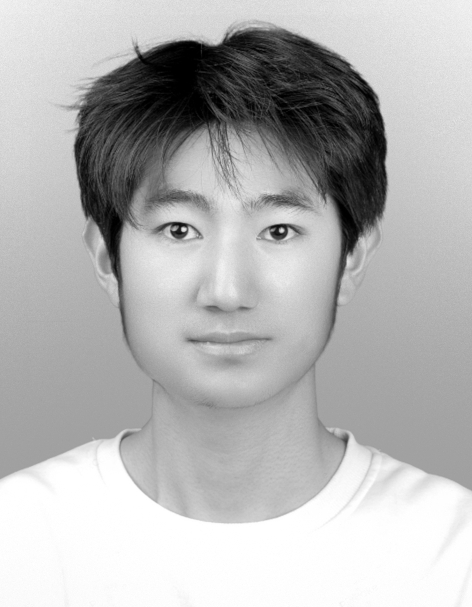
\includegraphics[height=2in,width=1in,clip,keepaspectratio]{ShuolongChen_grey.jpg}}
	 \noindent{\bfseries Shuolong Chen}\emph{
	 received the B.S. degree in geodesy and geomatics engineering from Wuhan University, Wuhan China, in 2023.
	 He is currently a master candidate at the school of Geodesy and Geomatics, Wuhan University. His area of research currently focuses on integrated navigation systems and multi-sensor fusion.
	 Contact him via e-mail: shlchen@whu.edu.cn.
	 }}
	\end{tcolorbox}
		
		
\end{document}
